% =====================================================================
%  Week 3 Implementation — New Policies, Retrieval Types & Gate Calibration
%  drop-in chapter section for the dissertation
%  Project: Adaptive Retrieval Gating for Safety-Aware Medical RAG
%  Author:  Tharit Mohamed Hussain Khan (22058691), KCL MSc AI, 7CCSMPRJ
%
%  To include in the main report:  % =====================================================================
%  Week 3 Implementation — New Policies, Retrieval Types & Gate Calibration
%  drop-in chapter section for the dissertation
%  Project: Adaptive Retrieval Gating for Safety-Aware Medical RAG
%  Author:  Tharit Mohamed Hussain Khan (22058691), KCL MSc AI, 7CCSMPRJ
%
%  To include in the main report:  % =====================================================================
%  Week 3 Implementation — New Policies, Retrieval Types & Gate Calibration
%  drop-in chapter section for the dissertation
%  Project: Adaptive Retrieval Gating for Safety-Aware Medical RAG
%  Author:  Tharit Mohamed Hussain Khan (22058691), KCL MSc AI, 7CCSMPRJ
%
%  To include in the main report:  % =====================================================================
%  Week 3 Implementation — New Policies, Retrieval Types & Gate Calibration
%  drop-in chapter section for the dissertation
%  Project: Adaptive Retrieval Gating for Safety-Aware Medical RAG
%  Author:  Tharit Mohamed Hussain Khan (22058691), KCL MSc AI, 7CCSMPRJ
%
%  To include in the main report:  \input{week3_policies}
%  Required preamble packages (shared with the other chapters):
%    \usepackage{booktabs} \usepackage{amsmath} \usepackage{amssymb}
%    \usepackage{graphicx}
%  Figures referenced live in results/figures/ (PNG + PDF both written).
% =====================================================================

\section{New Policies, Retrieval Types and Gate Calibration (Week 3)}
\label{sec:impl-week3}

Week~2 delivered the gating mechanism but left three gaps: the retrieval engine
was lexical-only (BM25), two of the six policies (P2, P4) were unimplemented, and
the gate thresholds were empirically shown never to fire on the quantised model.
This section documents closing all three. First, the semantic (vector) and hybrid
retrievers are added so that policies can retrieve on meaning rather than keyword
overlap alone. Second, policies P2 (always-retrieve with citations) and P4 (hybrid
retrieval) are implemented on top of the existing always-retrieve machinery.
Third, and most importantly, the gate thresholds are \emph{calibrated} to the
model's actual signal distribution, turning the selective policy~(P5) from a
degenerate always-skip system into one that genuinely routes per query. The
section closes with the first full comparison of all policies across both
multiple-choice and open-ended question types.

% ---------------------------------------------------------------------
\subsection{Semantic and Hybrid Retrieval}
\label{sec:retrieval-types}

The Week~2 pipeline retrieved with BM25 only. BM25 scores documents by lexical
overlap, so it misses paraphrase: a query about a \emph{heart attack} does not
match a passage that only ever says \emph{myocardial infarction}. Two additional
retrievers close this gap.

\paragraph{Vector retriever.} Each corpus chunk is embedded once with
\texttt{all-MiniLM-L6-v2} (384-dimensional) and indexed in a FAISS
\texttt{IndexFlatIP}. Because the embeddings are L2-normalised, inner product
equals cosine similarity, and \texttt{IndexFlatIP} is an \emph{exact} (brute-force)
index, so retrieval is deterministic and needs no training --- a deliberate choice
given the project's reproducibility and CPU-only constraints. At query time the
question is embedded with the same model and the top-$k$ chunks are returned by
cosine similarity. This retrieves on semantic proximity, catching the paraphrase
cases BM25 misses.

\paragraph{Hybrid retriever.} Lexical and semantic retrieval have complementary
strengths --- BM25 is precise on exact terminology (drug names, dosages), the
vector index generalises across wording. The hybrid retriever runs both and fuses
their rankings with Reciprocal Rank Fusion (RRF):
%
\begin{equation}
  \mathrm{score}(d) \;=\; \sum_{i \in \{\text{bm25},\,\text{vec}\}}
  \frac{1}{k + \mathrm{rank}_i(d)}, \qquad k = 60,
  \label{eq:rrf}
\end{equation}
%
where $\mathrm{rank}_i(d)$ is the 1-based rank of document $d$ in retriever $i$.
RRF is score-agnostic: it fuses \emph{ranks}, so the incomparable BM25 and cosine
scales never need normalising. Documents ranked highly by both retrievers rise to
the top; a document ranked first by both scores $2/61$. The constant $k=60$ is the
standard RRF damping value and is exposed as configuration.

A single factory selects the retriever from \texttt{cfg.policy.retrieval\_mode}
$\in\{\text{none},\text{bm25},\text{vector},\text{hybrid}\}$, so a policy's
retrieval strategy is a configuration choice, not a code change. The same policy
harness therefore runs unchanged across all four modes.

% ---------------------------------------------------------------------
\subsection{Policies P2 (Citations) and P4 (Hybrid)}
\label{sec:p2-p4}

\paragraph{P2 --- always retrieve with citations.} P2 extends the always-retrieve
baseline with provenance. The retrieval-augmented prompt asks the model to end its
answer with a \texttt{SOURCES:} line naming the passages it used; the policy parses
that line and matches the named titles back to the retrieved chunks, producing
\texttt{Citation} objects. Matching is deliberately lenient (case-insensitive
substring) because small models paraphrase titles, and any cited source that
matches no retrieved chunk is dropped --- an invented citation is not counted.
The matched citations feed citation precision/recall (cited~$\cap$~retrieved),
the attribution metric against which the gated policies are later judged.

\paragraph{P4 --- hybrid retrieval.} P4 is the always-retrieve policy bound to the
hybrid (RRF) retriever. Mechanically its answering step is identical to P1 ---
retrieve, build a RAG prompt, answer --- so it subclasses the always-retrieve
behaviour and differs only in the retriever the factory supplies. Keeping it a
distinct class makes the policy explicit in the logs and gives a home for any
future BM25-versus-vector routing logic.

% ---------------------------------------------------------------------
\subsection{Gate Calibration: Why the Defaults Never Fired}
\label{sec:calibration}

Week~2 reported a striking result: with the default thresholds
($\tau_H = 2.5$ nats for entropy, $\tau_M = 0.3$ for the logit margin) the gate
retrieved on \emph{zero} of 200 questions, so P5 collapsed onto the closed-book
policy P3. Section~\ref{sec:calibration} explains and fixes this.

The cause is that the default thresholds were never physically reachable for this
quantised 3B model. Figure~\ref{fig:signals} plots the logged per-query signals
against the thresholds. The entropy of the draft answer never exceeds
$\approx 1.6$ nats, so the ``retrieve if entropy $> 2.5$'' rule can never trigger;
symmetrically the margin never falls below $\approx 0.45$, so ``retrieve if
margin $< 0.3$'' can never trigger. Only the text-only hallucination probe ever
voted to retrieve, and under the 2-of-3 majority a lone vote is always outvoted.
The thresholds, taken from the literature on full-precision models, simply do not
transfer to a 4-bit quantised model --- a finding in its own right.

\begin{figure}[t]
  \centering
  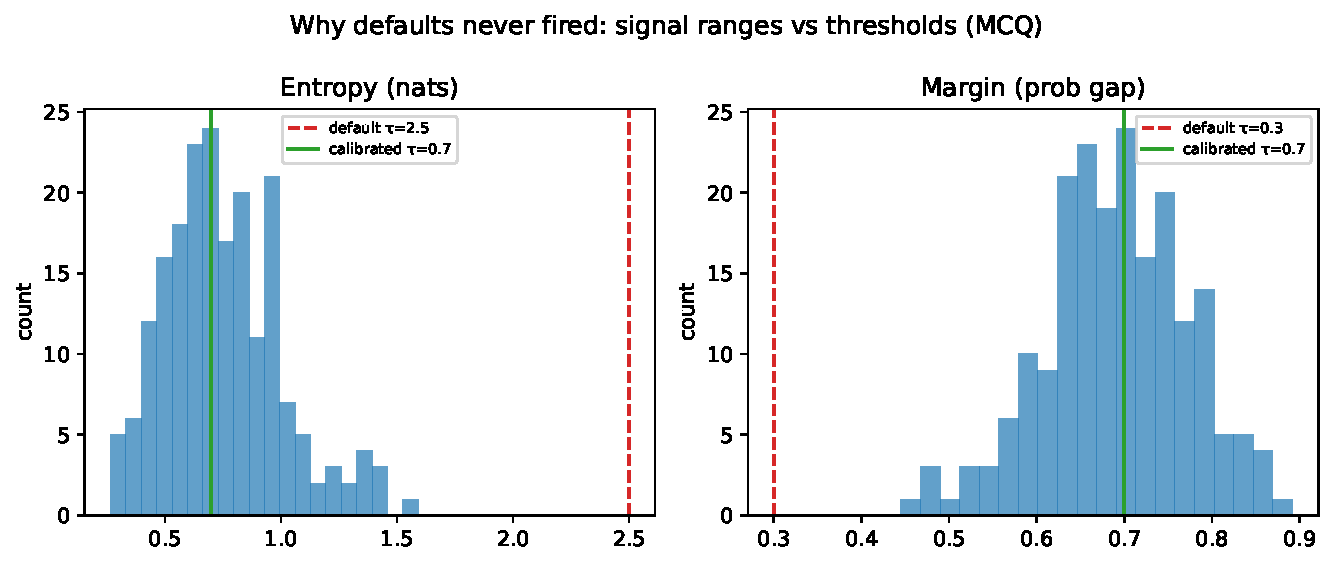
\includegraphics[width=\linewidth]{results/figures/fig_signals}
  \caption{Gate-signal distributions on 200 MIRAGE MCQs versus the thresholds.
  The default thresholds (red) lie entirely outside the observed signal range in
  both cases, so neither the entropy nor the margin gate could ever fire; the
  calibrated thresholds (green, $\tau=0.70$) sit within the signal mass.}
  \label{fig:signals}
\end{figure}

Calibration is performed \emph{offline}. Because every P5 run logs the raw
per-gate signal for every query, the retrieve/skip decision can be replayed at any
threshold without re-invoking the model. A sweep script
(\texttt{run\_threshold\_sweep.py}) reconstructs the ensemble decision over a grid
of thresholds in seconds rather than the hours a live re-run would cost. Choosing a
single global operating point $\tau_H = \tau_M = 0.70$ places the retrieval rate in
a sensible band for both question types (Figure~\ref{fig:retrieval}): roughly
$50\%$ on the multiple-choice set and $79\%$ on the open-ended set. The higher
open-ended rate is itself informative --- the probe's draft-agreement signal
disagrees far more often on free-text answers than on multiple-choice letters, so
the ensemble reaches the retrieve threshold more readily.

\begin{figure}[t]
  \centering
  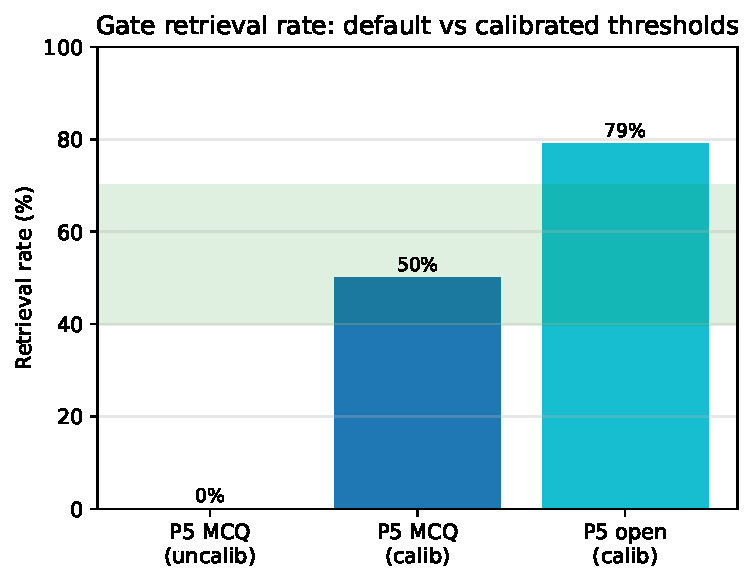
\includegraphics[width=0.75\linewidth]{results/figures/fig_retrieval}
  \caption{Gate retrieval rate before and after calibration. At default thresholds
  P5 retrieved on 0\% of queries; after calibration it retrieves at 50\% (MCQ) and
  79\% (open-ended), both within or above the 40--70\% target band (shaded).}
  \label{fig:retrieval}
\end{figure}

% ---------------------------------------------------------------------
\subsection{Open-Ended Evaluation}
\label{sec:open-ended}

All five MIRAGE subsets are multiple-choice, so the benchmark alone cannot test
free-text answering. The intended open-ended source (RAGCare-QA) was no longer
retrievable from its published location, so it was substituted with PubMedQA
(\texttt{pqa\_labeled}): 1{,}000 expert-annotated biomedical research questions,
each with a paragraph \emph{long answer}. This is genuine free-text question
answering, scored by token-level F1 (SQuAD-style) rather than letter matching, and
it exercises the hallucination probe's F1-agreement mode rather than its
letter-match mode. Both scoring and gating therefore branch correctly on question
type, verified end-to-end on the real data before any full run.

% ---------------------------------------------------------------------
\subsection{Results and the Headline Finding}
\label{sec:week3-results}

Table~\ref{tab:week3-results} reports all completed runs on the 200-question sets.
Two results stand out. First, calibration works exactly as designed: P5's
retrieval rate moves from 0\% to 50\% (MCQ) and 79\% (open-ended). Second, and
more consequentially, \emph{once P5 begins retrieving on the pilot corpus its
multiple-choice accuracy falls} from ccPthreeMcq{} (identical to closed-book, when it
never retrieved) to 45.5\%.

\begin{table}[t]
  \centering
  \begin{tabular}{lccccc}
    \toprule
    Policy & Type & $n$ & Acc.\ / F1 & Retrieval & Latency/q \\
    \midrule
    P1 always-retrieve   & MCQ  & 200 & 17.0\%          & 100\% & 12\,s \\
    P3 closed-book       & MCQ  & 200 & ccPthreeMcq   & 
etPthreeMcq & \latPthreeMcq \\
    P5 gated (uncalib.)  & MCQ  & 200 & ccPthreeMcq   & 0\%   & 142\,s \\
    P5 gated (calibrated)& MCQ  & 200 & 45.5\%          & 50\%  & 159\,s \\
    \midrule
    P3 closed-book       & open & 200 & 1PthreeOpen (F1) & 
etPthreeOpen & 27\,s \\
    P5 gated (calibrated)& open & 200 & 0.191 (F1)      & 79\%  & 171\,s \\
    \bottomrule
  \end{tabular}
  \caption{All completed 200-question runs (quantised Llama-3.2-3B, medium tier,
  200-chunk \emph{pilot} corpus). MCQ scored by accuracy, open-ended by mean
  token-F1. Latency is the mean wall-clock time per query.}
  \label{tab:week3-results}
\end{table}

This is not a bug but the central empirical finding: \textbf{gated retrieval
inherits the quality of the corpus it retrieves from}. The same effect explains
P1's very low 17.0\%: retrieving irrelevant context from a small pilot corpus
actively misleads the model relative to answering from its own parametric
knowledge, and the RAG prompt's instruction to rely on the provided context
compounds this. The gate is functioning correctly --- it fires at the calibrated
rate --- but on a weak corpus the act of retrieving is itself harmful. The
accuracy/latency frontier in Figure~\ref{fig:pareto} makes the trade-off concrete:
on the pilot corpus, closed-book (P3) dominates, being both cheaper and more
accurate than either retrieving policy.

\begin{figure}[t]
  \centering
  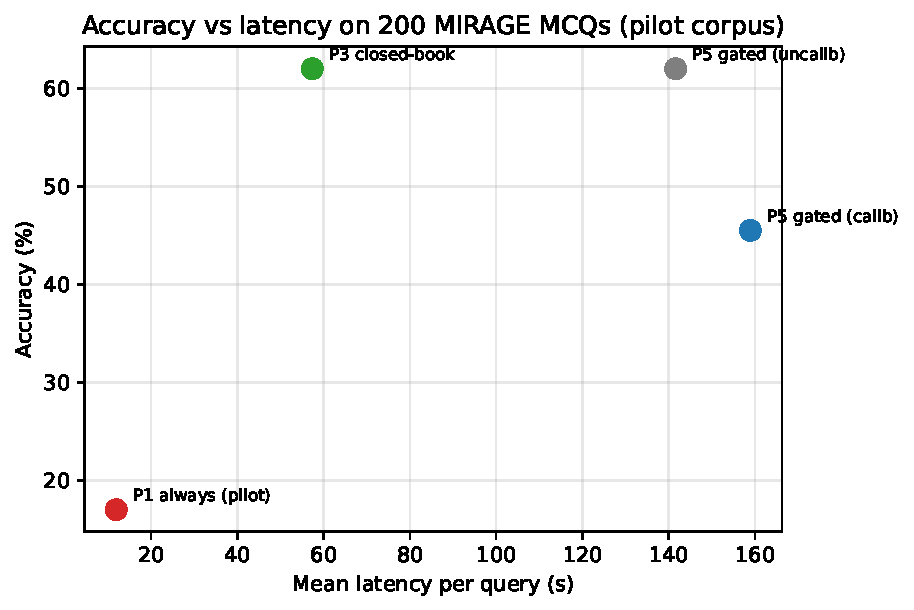
\includegraphics[width=0.8\linewidth]{results/figures/fig_pareto}
  \caption{Accuracy versus mean latency on 200 MIRAGE MCQs (pilot corpus). P3
  closed-book dominates the pilot-corpus frontier; the retrieving policies (P1,
  calibrated P5) pay a latency cost \emph{and} lose accuracy because pilot-corpus
  retrieval is unhelpful.}
  \label{fig:pareto}
\end{figure}

The practical consequence for the project is that the retrieval corpus, not the
gate, is now the critical variable: the gating machinery cannot be fairly evaluated
until it retrieves from a corpus that actually contains the answers. This directly
motivates the next phase --- replacing the pilot corpus with a real clinical
corpus (StatPearls / MedCorp) --- and reframes the safety-envelope analysis around
the corpus-quality dimension. It is also a genuinely useful negative result:
adaptive retrieval is only as safe as what it retrieves, and on a poor corpus the
safest gate is one that retrieves \emph{less}.

% ---------------------------------------------------------------------
\subsection{Summary}
\label{sec:week3-summary}

This sprint completed the retrieval engine (vector and hybrid retrievers),
implemented the remaining non-gated policies (P2, P4), and --- most importantly ---
calibrated the gate so that P5 performs genuine per-query routing. The full
cross-type comparison surfaced the project's headline finding: on the current
pilot corpus, retrieval degrades accuracy, so the corpus becomes the next
critical-path dependency. All figures and the results table are generated directly
from the logged per-query records, so the reported numbers and the plots share a
single source of truth.

%  Required preamble packages (shared with the other chapters):
%    \usepackage{booktabs} \usepackage{amsmath} \usepackage{amssymb}
%    \usepackage{graphicx}
%  Figures referenced live in results/figures/ (PNG + PDF both written).
% =====================================================================

\section{New Policies, Retrieval Types and Gate Calibration (Week 3)}
\label{sec:impl-week3}

Week~2 delivered the gating mechanism but left three gaps: the retrieval engine
was lexical-only (BM25), two of the six policies (P2, P4) were unimplemented, and
the gate thresholds were empirically shown never to fire on the quantised model.
This section documents closing all three. First, the semantic (vector) and hybrid
retrievers are added so that policies can retrieve on meaning rather than keyword
overlap alone. Second, policies P2 (always-retrieve with citations) and P4 (hybrid
retrieval) are implemented on top of the existing always-retrieve machinery.
Third, and most importantly, the gate thresholds are \emph{calibrated} to the
model's actual signal distribution, turning the selective policy~(P5) from a
degenerate always-skip system into one that genuinely routes per query. The
section closes with the first full comparison of all policies across both
multiple-choice and open-ended question types.

% ---------------------------------------------------------------------
\subsection{Semantic and Hybrid Retrieval}
\label{sec:retrieval-types}

The Week~2 pipeline retrieved with BM25 only. BM25 scores documents by lexical
overlap, so it misses paraphrase: a query about a \emph{heart attack} does not
match a passage that only ever says \emph{myocardial infarction}. Two additional
retrievers close this gap.

\paragraph{Vector retriever.} Each corpus chunk is embedded once with
\texttt{all-MiniLM-L6-v2} (384-dimensional) and indexed in a FAISS
\texttt{IndexFlatIP}. Because the embeddings are L2-normalised, inner product
equals cosine similarity, and \texttt{IndexFlatIP} is an \emph{exact} (brute-force)
index, so retrieval is deterministic and needs no training --- a deliberate choice
given the project's reproducibility and CPU-only constraints. At query time the
question is embedded with the same model and the top-$k$ chunks are returned by
cosine similarity. This retrieves on semantic proximity, catching the paraphrase
cases BM25 misses.

\paragraph{Hybrid retriever.} Lexical and semantic retrieval have complementary
strengths --- BM25 is precise on exact terminology (drug names, dosages), the
vector index generalises across wording. The hybrid retriever runs both and fuses
their rankings with Reciprocal Rank Fusion (RRF):
%
\begin{equation}
  \mathrm{score}(d) \;=\; \sum_{i \in \{\text{bm25},\,\text{vec}\}}
  \frac{1}{k + \mathrm{rank}_i(d)}, \qquad k = 60,
  \label{eq:rrf}
\end{equation}
%
where $\mathrm{rank}_i(d)$ is the 1-based rank of document $d$ in retriever $i$.
RRF is score-agnostic: it fuses \emph{ranks}, so the incomparable BM25 and cosine
scales never need normalising. Documents ranked highly by both retrievers rise to
the top; a document ranked first by both scores $2/61$. The constant $k=60$ is the
standard RRF damping value and is exposed as configuration.

A single factory selects the retriever from \texttt{cfg.policy.retrieval\_mode}
$\in\{\text{none},\text{bm25},\text{vector},\text{hybrid}\}$, so a policy's
retrieval strategy is a configuration choice, not a code change. The same policy
harness therefore runs unchanged across all four modes.

% ---------------------------------------------------------------------
\subsection{Policies P2 (Citations) and P4 (Hybrid)}
\label{sec:p2-p4}

\paragraph{P2 --- always retrieve with citations.} P2 extends the always-retrieve
baseline with provenance. The retrieval-augmented prompt asks the model to end its
answer with a \texttt{SOURCES:} line naming the passages it used; the policy parses
that line and matches the named titles back to the retrieved chunks, producing
\texttt{Citation} objects. Matching is deliberately lenient (case-insensitive
substring) because small models paraphrase titles, and any cited source that
matches no retrieved chunk is dropped --- an invented citation is not counted.
The matched citations feed citation precision/recall (cited~$\cap$~retrieved),
the attribution metric against which the gated policies are later judged.

\paragraph{P4 --- hybrid retrieval.} P4 is the always-retrieve policy bound to the
hybrid (RRF) retriever. Mechanically its answering step is identical to P1 ---
retrieve, build a RAG prompt, answer --- so it subclasses the always-retrieve
behaviour and differs only in the retriever the factory supplies. Keeping it a
distinct class makes the policy explicit in the logs and gives a home for any
future BM25-versus-vector routing logic.

% ---------------------------------------------------------------------
\subsection{Gate Calibration: Why the Defaults Never Fired}
\label{sec:calibration}

Week~2 reported a striking result: with the default thresholds
($\tau_H = 2.5$ nats for entropy, $\tau_M = 0.3$ for the logit margin) the gate
retrieved on \emph{zero} of 200 questions, so P5 collapsed onto the closed-book
policy P3. Section~\ref{sec:calibration} explains and fixes this.

The cause is that the default thresholds were never physically reachable for this
quantised 3B model. Figure~\ref{fig:signals} plots the logged per-query signals
against the thresholds. The entropy of the draft answer never exceeds
$\approx 1.6$ nats, so the ``retrieve if entropy $> 2.5$'' rule can never trigger;
symmetrically the margin never falls below $\approx 0.45$, so ``retrieve if
margin $< 0.3$'' can never trigger. Only the text-only hallucination probe ever
voted to retrieve, and under the 2-of-3 majority a lone vote is always outvoted.
The thresholds, taken from the literature on full-precision models, simply do not
transfer to a 4-bit quantised model --- a finding in its own right.

\begin{figure}[t]
  \centering
  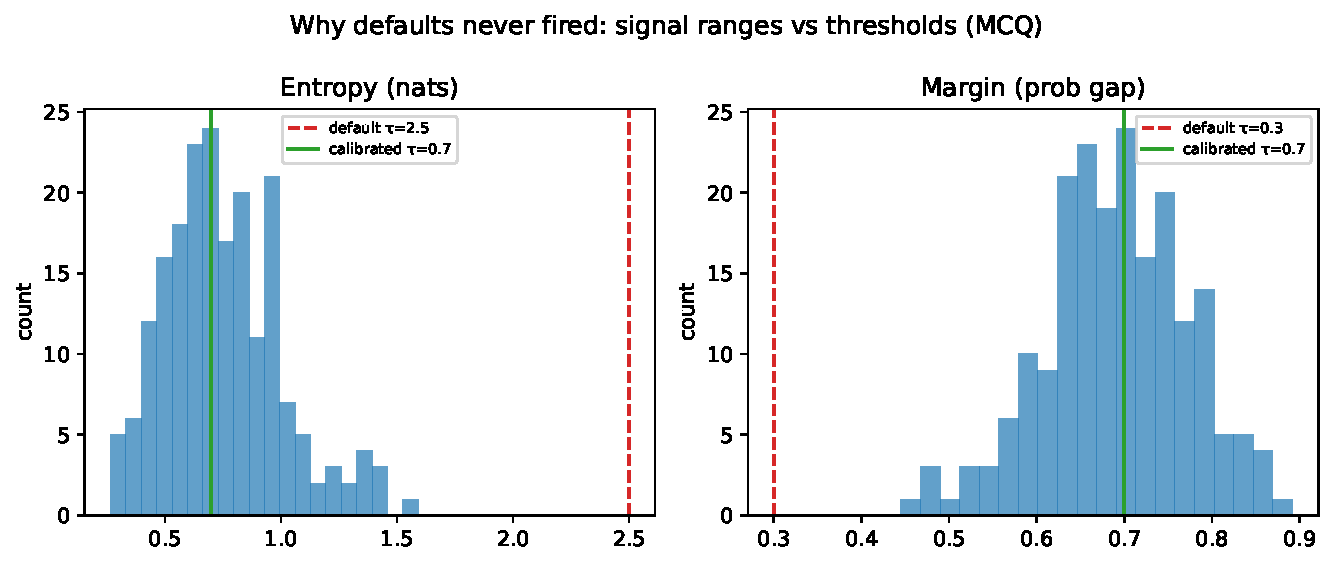
\includegraphics[width=\linewidth]{results/figures/fig_signals}
  \caption{Gate-signal distributions on 200 MIRAGE MCQs versus the thresholds.
  The default thresholds (red) lie entirely outside the observed signal range in
  both cases, so neither the entropy nor the margin gate could ever fire; the
  calibrated thresholds (green, $\tau=0.70$) sit within the signal mass.}
  \label{fig:signals}
\end{figure}

Calibration is performed \emph{offline}. Because every P5 run logs the raw
per-gate signal for every query, the retrieve/skip decision can be replayed at any
threshold without re-invoking the model. A sweep script
(\texttt{run\_threshold\_sweep.py}) reconstructs the ensemble decision over a grid
of thresholds in seconds rather than the hours a live re-run would cost. Choosing a
single global operating point $\tau_H = \tau_M = 0.70$ places the retrieval rate in
a sensible band for both question types (Figure~\ref{fig:retrieval}): roughly
$50\%$ on the multiple-choice set and $79\%$ on the open-ended set. The higher
open-ended rate is itself informative --- the probe's draft-agreement signal
disagrees far more often on free-text answers than on multiple-choice letters, so
the ensemble reaches the retrieve threshold more readily.

\begin{figure}[t]
  \centering
  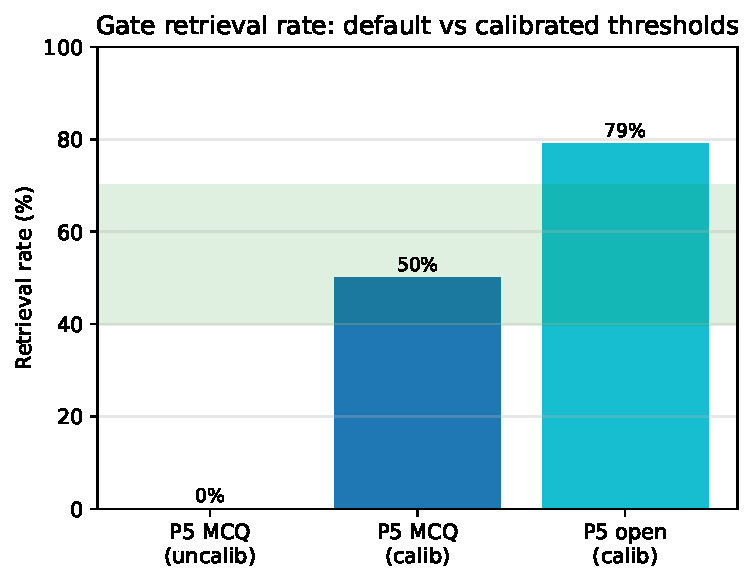
\includegraphics[width=0.75\linewidth]{results/figures/fig_retrieval}
  \caption{Gate retrieval rate before and after calibration. At default thresholds
  P5 retrieved on 0\% of queries; after calibration it retrieves at 50\% (MCQ) and
  79\% (open-ended), both within or above the 40--70\% target band (shaded).}
  \label{fig:retrieval}
\end{figure}

% ---------------------------------------------------------------------
\subsection{Open-Ended Evaluation}
\label{sec:open-ended}

All five MIRAGE subsets are multiple-choice, so the benchmark alone cannot test
free-text answering. The intended open-ended source (RAGCare-QA) was no longer
retrievable from its published location, so it was substituted with PubMedQA
(\texttt{pqa\_labeled}): 1{,}000 expert-annotated biomedical research questions,
each with a paragraph \emph{long answer}. This is genuine free-text question
answering, scored by token-level F1 (SQuAD-style) rather than letter matching, and
it exercises the hallucination probe's F1-agreement mode rather than its
letter-match mode. Both scoring and gating therefore branch correctly on question
type, verified end-to-end on the real data before any full run.

% ---------------------------------------------------------------------
\subsection{Results and the Headline Finding}
\label{sec:week3-results}

Table~\ref{tab:week3-results} reports all completed runs on the 200-question sets.
Two results stand out. First, calibration works exactly as designed: P5's
retrieval rate moves from 0\% to 50\% (MCQ) and 79\% (open-ended). Second, and
more consequentially, \emph{once P5 begins retrieving on the pilot corpus its
multiple-choice accuracy falls} from ccPthreeMcq{} (identical to closed-book, when it
never retrieved) to 45.5\%.

\begin{table}[t]
  \centering
  \begin{tabular}{lccccc}
    \toprule
    Policy & Type & $n$ & Acc.\ / F1 & Retrieval & Latency/q \\
    \midrule
    P1 always-retrieve   & MCQ  & 200 & 17.0\%          & 100\% & 12\,s \\
    P3 closed-book       & MCQ  & 200 & ccPthreeMcq   & 
etPthreeMcq & \latPthreeMcq \\
    P5 gated (uncalib.)  & MCQ  & 200 & ccPthreeMcq   & 0\%   & 142\,s \\
    P5 gated (calibrated)& MCQ  & 200 & 45.5\%          & 50\%  & 159\,s \\
    \midrule
    P3 closed-book       & open & 200 & 1PthreeOpen (F1) & 
etPthreeOpen & 27\,s \\
    P5 gated (calibrated)& open & 200 & 0.191 (F1)      & 79\%  & 171\,s \\
    \bottomrule
  \end{tabular}
  \caption{All completed 200-question runs (quantised Llama-3.2-3B, medium tier,
  200-chunk \emph{pilot} corpus). MCQ scored by accuracy, open-ended by mean
  token-F1. Latency is the mean wall-clock time per query.}
  \label{tab:week3-results}
\end{table}

This is not a bug but the central empirical finding: \textbf{gated retrieval
inherits the quality of the corpus it retrieves from}. The same effect explains
P1's very low 17.0\%: retrieving irrelevant context from a small pilot corpus
actively misleads the model relative to answering from its own parametric
knowledge, and the RAG prompt's instruction to rely on the provided context
compounds this. The gate is functioning correctly --- it fires at the calibrated
rate --- but on a weak corpus the act of retrieving is itself harmful. The
accuracy/latency frontier in Figure~\ref{fig:pareto} makes the trade-off concrete:
on the pilot corpus, closed-book (P3) dominates, being both cheaper and more
accurate than either retrieving policy.

\begin{figure}[t]
  \centering
  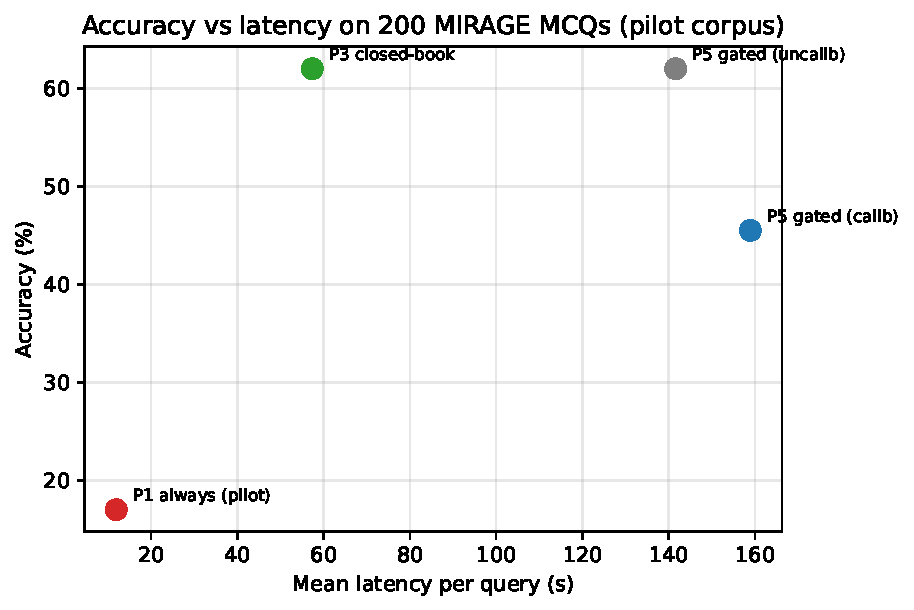
\includegraphics[width=0.8\linewidth]{results/figures/fig_pareto}
  \caption{Accuracy versus mean latency on 200 MIRAGE MCQs (pilot corpus). P3
  closed-book dominates the pilot-corpus frontier; the retrieving policies (P1,
  calibrated P5) pay a latency cost \emph{and} lose accuracy because pilot-corpus
  retrieval is unhelpful.}
  \label{fig:pareto}
\end{figure}

The practical consequence for the project is that the retrieval corpus, not the
gate, is now the critical variable: the gating machinery cannot be fairly evaluated
until it retrieves from a corpus that actually contains the answers. This directly
motivates the next phase --- replacing the pilot corpus with a real clinical
corpus (StatPearls / MedCorp) --- and reframes the safety-envelope analysis around
the corpus-quality dimension. It is also a genuinely useful negative result:
adaptive retrieval is only as safe as what it retrieves, and on a poor corpus the
safest gate is one that retrieves \emph{less}.

% ---------------------------------------------------------------------
\subsection{Summary}
\label{sec:week3-summary}

This sprint completed the retrieval engine (vector and hybrid retrievers),
implemented the remaining non-gated policies (P2, P4), and --- most importantly ---
calibrated the gate so that P5 performs genuine per-query routing. The full
cross-type comparison surfaced the project's headline finding: on the current
pilot corpus, retrieval degrades accuracy, so the corpus becomes the next
critical-path dependency. All figures and the results table are generated directly
from the logged per-query records, so the reported numbers and the plots share a
single source of truth.

%  Required preamble packages (shared with the other chapters):
%    \usepackage{booktabs} \usepackage{amsmath} \usepackage{amssymb}
%    \usepackage{graphicx}
%  Figures referenced live in results/figures/ (PNG + PDF both written).
% =====================================================================

\section{New Policies, Retrieval Types and Gate Calibration (Week 3)}
\label{sec:impl-week3}

Week~2 delivered the gating mechanism but left three gaps: the retrieval engine
was lexical-only (BM25), two of the six policies (P2, P4) were unimplemented, and
the gate thresholds were empirically shown never to fire on the quantised model.
This section documents closing all three. First, the semantic (vector) and hybrid
retrievers are added so that policies can retrieve on meaning rather than keyword
overlap alone. Second, policies P2 (always-retrieve with citations) and P4 (hybrid
retrieval) are implemented on top of the existing always-retrieve machinery.
Third, and most importantly, the gate thresholds are \emph{calibrated} to the
model's actual signal distribution, turning the selective policy~(P5) from a
degenerate always-skip system into one that genuinely routes per query. The
section closes with the first full comparison of all policies across both
multiple-choice and open-ended question types.

% ---------------------------------------------------------------------
\subsection{Semantic and Hybrid Retrieval}
\label{sec:retrieval-types}

The Week~2 pipeline retrieved with BM25 only. BM25 scores documents by lexical
overlap, so it misses paraphrase: a query about a \emph{heart attack} does not
match a passage that only ever says \emph{myocardial infarction}. Two additional
retrievers close this gap.

\paragraph{Vector retriever.} Each corpus chunk is embedded once with
\texttt{all-MiniLM-L6-v2} (384-dimensional) and indexed in a FAISS
\texttt{IndexFlatIP}. Because the embeddings are L2-normalised, inner product
equals cosine similarity, and \texttt{IndexFlatIP} is an \emph{exact} (brute-force)
index, so retrieval is deterministic and needs no training --- a deliberate choice
given the project's reproducibility and CPU-only constraints. At query time the
question is embedded with the same model and the top-$k$ chunks are returned by
cosine similarity. This retrieves on semantic proximity, catching the paraphrase
cases BM25 misses.

\paragraph{Hybrid retriever.} Lexical and semantic retrieval have complementary
strengths --- BM25 is precise on exact terminology (drug names, dosages), the
vector index generalises across wording. The hybrid retriever runs both and fuses
their rankings with Reciprocal Rank Fusion (RRF):
%
\begin{equation}
  \mathrm{score}(d) \;=\; \sum_{i \in \{\text{bm25},\,\text{vec}\}}
  \frac{1}{k + \mathrm{rank}_i(d)}, \qquad k = 60,
  \label{eq:rrf}
\end{equation}
%
where $\mathrm{rank}_i(d)$ is the 1-based rank of document $d$ in retriever $i$.
RRF is score-agnostic: it fuses \emph{ranks}, so the incomparable BM25 and cosine
scales never need normalising. Documents ranked highly by both retrievers rise to
the top; a document ranked first by both scores $2/61$. The constant $k=60$ is the
standard RRF damping value and is exposed as configuration.

A single factory selects the retriever from \texttt{cfg.policy.retrieval\_mode}
$\in\{\text{none},\text{bm25},\text{vector},\text{hybrid}\}$, so a policy's
retrieval strategy is a configuration choice, not a code change. The same policy
harness therefore runs unchanged across all four modes.

% ---------------------------------------------------------------------
\subsection{Policies P2 (Citations) and P4 (Hybrid)}
\label{sec:p2-p4}

\paragraph{P2 --- always retrieve with citations.} P2 extends the always-retrieve
baseline with provenance. The retrieval-augmented prompt asks the model to end its
answer with a \texttt{SOURCES:} line naming the passages it used; the policy parses
that line and matches the named titles back to the retrieved chunks, producing
\texttt{Citation} objects. Matching is deliberately lenient (case-insensitive
substring) because small models paraphrase titles, and any cited source that
matches no retrieved chunk is dropped --- an invented citation is not counted.
The matched citations feed citation precision/recall (cited~$\cap$~retrieved),
the attribution metric against which the gated policies are later judged.

\paragraph{P4 --- hybrid retrieval.} P4 is the always-retrieve policy bound to the
hybrid (RRF) retriever. Mechanically its answering step is identical to P1 ---
retrieve, build a RAG prompt, answer --- so it subclasses the always-retrieve
behaviour and differs only in the retriever the factory supplies. Keeping it a
distinct class makes the policy explicit in the logs and gives a home for any
future BM25-versus-vector routing logic.

% ---------------------------------------------------------------------
\subsection{Gate Calibration: Why the Defaults Never Fired}
\label{sec:calibration}

Week~2 reported a striking result: with the default thresholds
($\tau_H = 2.5$ nats for entropy, $\tau_M = 0.3$ for the logit margin) the gate
retrieved on \emph{zero} of 200 questions, so P5 collapsed onto the closed-book
policy P3. Section~\ref{sec:calibration} explains and fixes this.

The cause is that the default thresholds were never physically reachable for this
quantised 3B model. Figure~\ref{fig:signals} plots the logged per-query signals
against the thresholds. The entropy of the draft answer never exceeds
$\approx 1.6$ nats, so the ``retrieve if entropy $> 2.5$'' rule can never trigger;
symmetrically the margin never falls below $\approx 0.45$, so ``retrieve if
margin $< 0.3$'' can never trigger. Only the text-only hallucination probe ever
voted to retrieve, and under the 2-of-3 majority a lone vote is always outvoted.
The thresholds, taken from the literature on full-precision models, simply do not
transfer to a 4-bit quantised model --- a finding in its own right.

\begin{figure}[t]
  \centering
  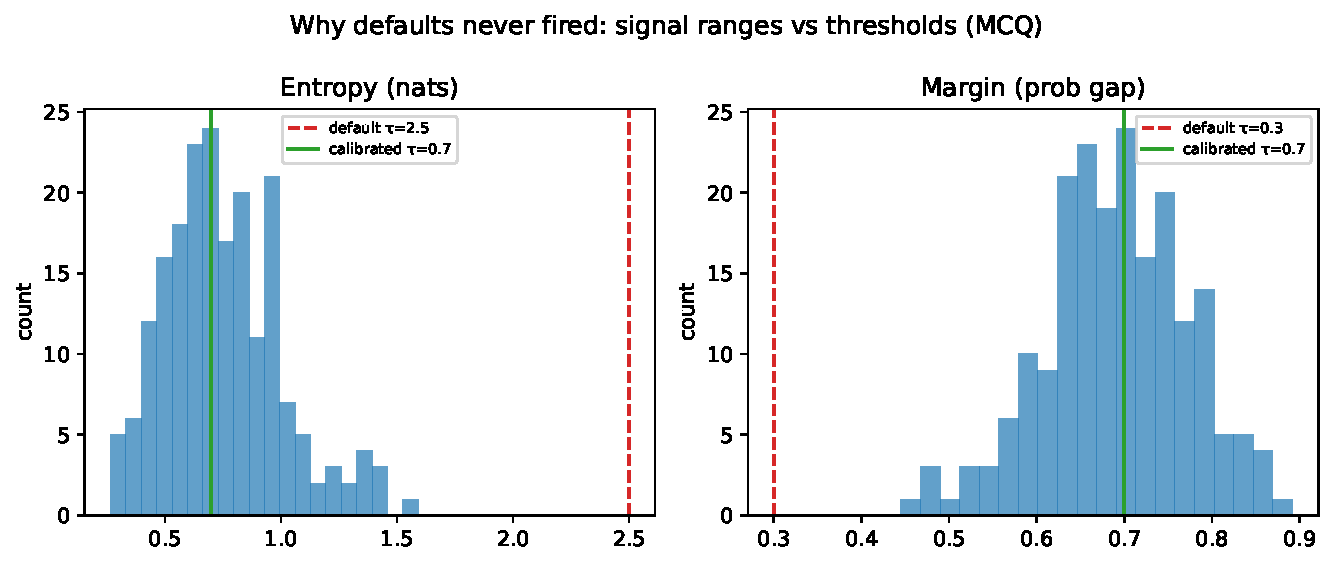
\includegraphics[width=\linewidth]{results/figures/fig_signals}
  \caption{Gate-signal distributions on 200 MIRAGE MCQs versus the thresholds.
  The default thresholds (red) lie entirely outside the observed signal range in
  both cases, so neither the entropy nor the margin gate could ever fire; the
  calibrated thresholds (green, $\tau=0.70$) sit within the signal mass.}
  \label{fig:signals}
\end{figure}

Calibration is performed \emph{offline}. Because every P5 run logs the raw
per-gate signal for every query, the retrieve/skip decision can be replayed at any
threshold without re-invoking the model. A sweep script
(\texttt{run\_threshold\_sweep.py}) reconstructs the ensemble decision over a grid
of thresholds in seconds rather than the hours a live re-run would cost. Choosing a
single global operating point $\tau_H = \tau_M = 0.70$ places the retrieval rate in
a sensible band for both question types (Figure~\ref{fig:retrieval}): roughly
$50\%$ on the multiple-choice set and $79\%$ on the open-ended set. The higher
open-ended rate is itself informative --- the probe's draft-agreement signal
disagrees far more often on free-text answers than on multiple-choice letters, so
the ensemble reaches the retrieve threshold more readily.

\begin{figure}[t]
  \centering
  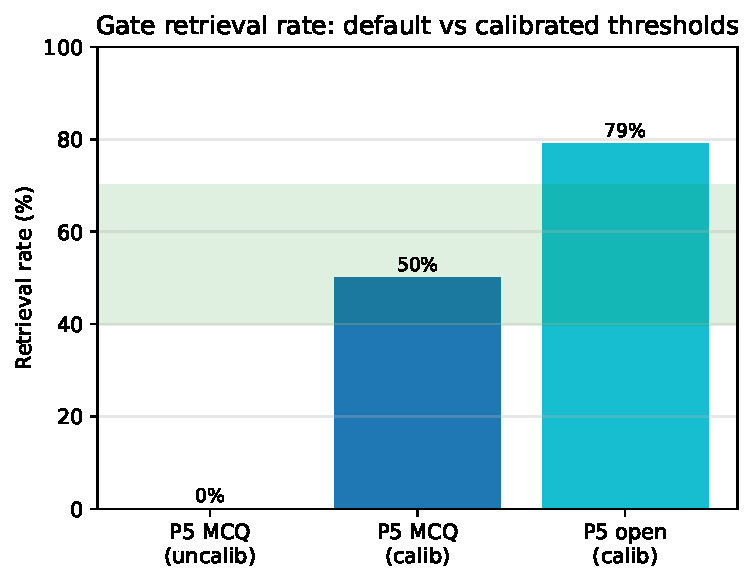
\includegraphics[width=0.75\linewidth]{results/figures/fig_retrieval}
  \caption{Gate retrieval rate before and after calibration. At default thresholds
  P5 retrieved on 0\% of queries; after calibration it retrieves at 50\% (MCQ) and
  79\% (open-ended), both within or above the 40--70\% target band (shaded).}
  \label{fig:retrieval}
\end{figure}

% ---------------------------------------------------------------------
\subsection{Open-Ended Evaluation}
\label{sec:open-ended}

All five MIRAGE subsets are multiple-choice, so the benchmark alone cannot test
free-text answering. The intended open-ended source (RAGCare-QA) was no longer
retrievable from its published location, so it was substituted with PubMedQA
(\texttt{pqa\_labeled}): 1{,}000 expert-annotated biomedical research questions,
each with a paragraph \emph{long answer}. This is genuine free-text question
answering, scored by token-level F1 (SQuAD-style) rather than letter matching, and
it exercises the hallucination probe's F1-agreement mode rather than its
letter-match mode. Both scoring and gating therefore branch correctly on question
type, verified end-to-end on the real data before any full run.

% ---------------------------------------------------------------------
\subsection{Results and the Headline Finding}
\label{sec:week3-results}

Table~\ref{tab:week3-results} reports all completed runs on the 200-question sets.
Two results stand out. First, calibration works exactly as designed: P5's
retrieval rate moves from 0\% to 50\% (MCQ) and 79\% (open-ended). Second, and
more consequentially, \emph{once P5 begins retrieving on the pilot corpus its
multiple-choice accuracy falls} from ccPthreeMcq{} (identical to closed-book, when it
never retrieved) to 45.5\%.

\begin{table}[t]
  \centering
  \begin{tabular}{lccccc}
    \toprule
    Policy & Type & $n$ & Acc.\ / F1 & Retrieval & Latency/q \\
    \midrule
    P1 always-retrieve   & MCQ  & 200 & 17.0\%          & 100\% & 12\,s \\
    P3 closed-book       & MCQ  & 200 & ccPthreeMcq   & 
etPthreeMcq & \latPthreeMcq \\
    P5 gated (uncalib.)  & MCQ  & 200 & ccPthreeMcq   & 0\%   & 142\,s \\
    P5 gated (calibrated)& MCQ  & 200 & 45.5\%          & 50\%  & 159\,s \\
    \midrule
    P3 closed-book       & open & 200 & 1PthreeOpen (F1) & 
etPthreeOpen & 27\,s \\
    P5 gated (calibrated)& open & 200 & 0.191 (F1)      & 79\%  & 171\,s \\
    \bottomrule
  \end{tabular}
  \caption{All completed 200-question runs (quantised Llama-3.2-3B, medium tier,
  200-chunk \emph{pilot} corpus). MCQ scored by accuracy, open-ended by mean
  token-F1. Latency is the mean wall-clock time per query.}
  \label{tab:week3-results}
\end{table}

This is not a bug but the central empirical finding: \textbf{gated retrieval
inherits the quality of the corpus it retrieves from}. The same effect explains
P1's very low 17.0\%: retrieving irrelevant context from a small pilot corpus
actively misleads the model relative to answering from its own parametric
knowledge, and the RAG prompt's instruction to rely on the provided context
compounds this. The gate is functioning correctly --- it fires at the calibrated
rate --- but on a weak corpus the act of retrieving is itself harmful. The
accuracy/latency frontier in Figure~\ref{fig:pareto} makes the trade-off concrete:
on the pilot corpus, closed-book (P3) dominates, being both cheaper and more
accurate than either retrieving policy.

\begin{figure}[t]
  \centering
  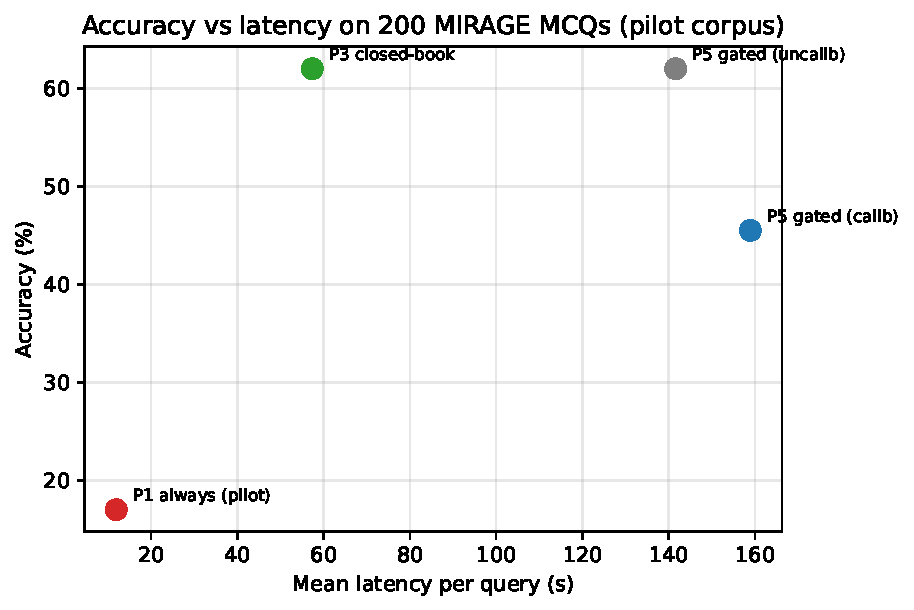
\includegraphics[width=0.8\linewidth]{results/figures/fig_pareto}
  \caption{Accuracy versus mean latency on 200 MIRAGE MCQs (pilot corpus). P3
  closed-book dominates the pilot-corpus frontier; the retrieving policies (P1,
  calibrated P5) pay a latency cost \emph{and} lose accuracy because pilot-corpus
  retrieval is unhelpful.}
  \label{fig:pareto}
\end{figure}

The practical consequence for the project is that the retrieval corpus, not the
gate, is now the critical variable: the gating machinery cannot be fairly evaluated
until it retrieves from a corpus that actually contains the answers. This directly
motivates the next phase --- replacing the pilot corpus with a real clinical
corpus (StatPearls / MedCorp) --- and reframes the safety-envelope analysis around
the corpus-quality dimension. It is also a genuinely useful negative result:
adaptive retrieval is only as safe as what it retrieves, and on a poor corpus the
safest gate is one that retrieves \emph{less}.

% ---------------------------------------------------------------------
\subsection{Summary}
\label{sec:week3-summary}

This sprint completed the retrieval engine (vector and hybrid retrievers),
implemented the remaining non-gated policies (P2, P4), and --- most importantly ---
calibrated the gate so that P5 performs genuine per-query routing. The full
cross-type comparison surfaced the project's headline finding: on the current
pilot corpus, retrieval degrades accuracy, so the corpus becomes the next
critical-path dependency. All figures and the results table are generated directly
from the logged per-query records, so the reported numbers and the plots share a
single source of truth.

%  Required preamble packages (shared with the other chapters):
%    \usepackage{booktabs} \usepackage{amsmath} \usepackage{amssymb}
%    \usepackage{graphicx}
%  Figures referenced live in results/figures/ (PNG + PDF both written).
% =====================================================================

\section{New Policies, Retrieval Types and Gate Calibration (Week 3)}
\label{sec:impl-week3}

Week~2 delivered the gating mechanism but left three gaps: the retrieval engine
was lexical-only (BM25), two of the six policies (P2, P4) were unimplemented, and
the gate thresholds were empirically shown never to fire on the quantised model.
This section documents closing all three. First, the semantic (vector) and hybrid
retrievers are added so that policies can retrieve on meaning rather than keyword
overlap alone. Second, policies P2 (always-retrieve with citations) and P4 (hybrid
retrieval) are implemented on top of the existing always-retrieve machinery.
Third, and most importantly, the gate thresholds are \emph{calibrated} to the
model's actual signal distribution, turning the selective policy~(P5) from a
degenerate always-skip system into one that genuinely routes per query. The
section closes with the first full comparison of all policies across both
multiple-choice and open-ended question types.

% ---------------------------------------------------------------------
\subsection{Semantic and Hybrid Retrieval}
\label{sec:retrieval-types}

The Week~2 pipeline retrieved with BM25 only. BM25 scores documents by lexical
overlap, so it misses paraphrase: a query about a \emph{heart attack} does not
match a passage that only ever says \emph{myocardial infarction}. Two additional
retrievers close this gap.

\paragraph{Vector retriever.} Each corpus chunk is embedded once with
\texttt{all-MiniLM-L6-v2} (384-dimensional) and indexed in a FAISS
\texttt{IndexFlatIP}. Because the embeddings are L2-normalised, inner product
equals cosine similarity, and \texttt{IndexFlatIP} is an \emph{exact} (brute-force)
index, so retrieval is deterministic and needs no training --- a deliberate choice
given the project's reproducibility and CPU-only constraints. At query time the
question is embedded with the same model and the top-$k$ chunks are returned by
cosine similarity. This retrieves on semantic proximity, catching the paraphrase
cases BM25 misses.

\paragraph{Hybrid retriever.} Lexical and semantic retrieval have complementary
strengths --- BM25 is precise on exact terminology (drug names, dosages), the
vector index generalises across wording. The hybrid retriever runs both and fuses
their rankings with Reciprocal Rank Fusion (RRF):
%
\begin{equation}
  \mathrm{score}(d) \;=\; \sum_{i \in \{\text{bm25},\,\text{vec}\}}
  \frac{1}{k + \mathrm{rank}_i(d)}, \qquad k = 60,
  \label{eq:rrf}
\end{equation}
%
where $\mathrm{rank}_i(d)$ is the 1-based rank of document $d$ in retriever $i$.
RRF is score-agnostic: it fuses \emph{ranks}, so the incomparable BM25 and cosine
scales never need normalising. Documents ranked highly by both retrievers rise to
the top; a document ranked first by both scores $2/61$. The constant $k=60$ is the
standard RRF damping value and is exposed as configuration.

A single factory selects the retriever from \texttt{cfg.policy.retrieval\_mode}
$\in\{\text{none},\text{bm25},\text{vector},\text{hybrid}\}$, so a policy's
retrieval strategy is a configuration choice, not a code change. The same policy
harness therefore runs unchanged across all four modes.

% ---------------------------------------------------------------------
\subsection{Policies P2 (Citations) and P4 (Hybrid)}
\label{sec:p2-p4}

\paragraph{P2 --- always retrieve with citations.} P2 extends the always-retrieve
baseline with provenance. The retrieval-augmented prompt asks the model to end its
answer with a \texttt{SOURCES:} line naming the passages it used; the policy parses
that line and matches the named titles back to the retrieved chunks, producing
\texttt{Citation} objects. Matching is deliberately lenient (case-insensitive
substring) because small models paraphrase titles, and any cited source that
matches no retrieved chunk is dropped --- an invented citation is not counted.
The matched citations feed citation precision/recall (cited~$\cap$~retrieved),
the attribution metric against which the gated policies are later judged.

\paragraph{P4 --- hybrid retrieval.} P4 is the always-retrieve policy bound to the
hybrid (RRF) retriever. Mechanically its answering step is identical to P1 ---
retrieve, build a RAG prompt, answer --- so it subclasses the always-retrieve
behaviour and differs only in the retriever the factory supplies. Keeping it a
distinct class makes the policy explicit in the logs and gives a home for any
future BM25-versus-vector routing logic.

% ---------------------------------------------------------------------
\subsection{Gate Calibration: Why the Defaults Never Fired}
\label{sec:calibration}

Week~2 reported a striking result: with the default thresholds
($\tau_H = 2.5$ nats for entropy, $\tau_M = 0.3$ for the logit margin) the gate
retrieved on \emph{zero} of 200 questions, so P5 collapsed onto the closed-book
policy P3. Section~\ref{sec:calibration} explains and fixes this.

The cause is that the default thresholds were never physically reachable for this
quantised 3B model. Figure~\ref{fig:signals} plots the logged per-query signals
against the thresholds. The entropy of the draft answer never exceeds
$\approx 1.6$ nats, so the ``retrieve if entropy $> 2.5$'' rule can never trigger;
symmetrically the margin never falls below $\approx 0.45$, so ``retrieve if
margin $< 0.3$'' can never trigger. Only the text-only hallucination probe ever
voted to retrieve, and under the 2-of-3 majority a lone vote is always outvoted.
The thresholds, taken from the literature on full-precision models, simply do not
transfer to a 4-bit quantised model --- a finding in its own right.

\begin{figure}[t]
  \centering
  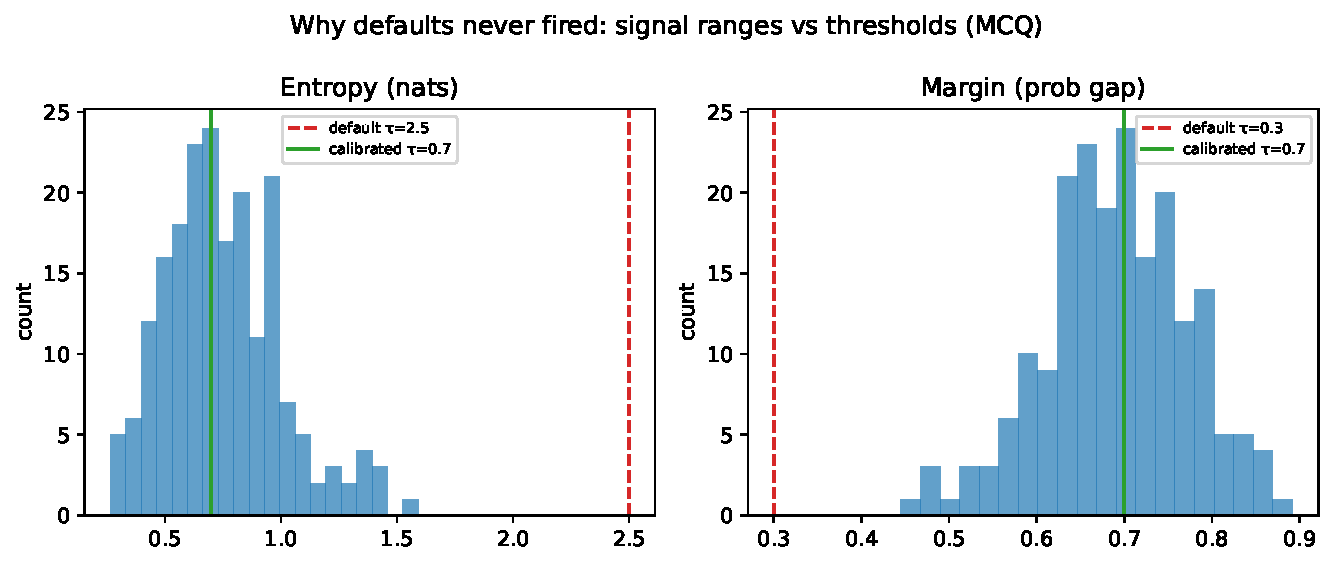
\includegraphics[width=\linewidth]{results/figures/fig_signals}
  \caption{Gate-signal distributions on 200 MIRAGE MCQs versus the thresholds.
  The default thresholds (red) lie entirely outside the observed signal range in
  both cases, so neither the entropy nor the margin gate could ever fire; the
  calibrated thresholds (green, $\tau=0.70$) sit within the signal mass.}
  \label{fig:signals}
\end{figure}

Calibration is performed \emph{offline}. Because every P5 run logs the raw
per-gate signal for every query, the retrieve/skip decision can be replayed at any
threshold without re-invoking the model. A sweep script
(\texttt{run\_threshold\_sweep.py}) reconstructs the ensemble decision over a grid
of thresholds in seconds rather than the hours a live re-run would cost. Choosing a
single global operating point $\tau_H = \tau_M = 0.70$ places the retrieval rate in
a sensible band for both question types (Figure~\ref{fig:retrieval}): roughly
$50\%$ on the multiple-choice set and $79\%$ on the open-ended set. The higher
open-ended rate is itself informative --- the probe's draft-agreement signal
disagrees far more often on free-text answers than on multiple-choice letters, so
the ensemble reaches the retrieve threshold more readily.

\begin{figure}[t]
  \centering
  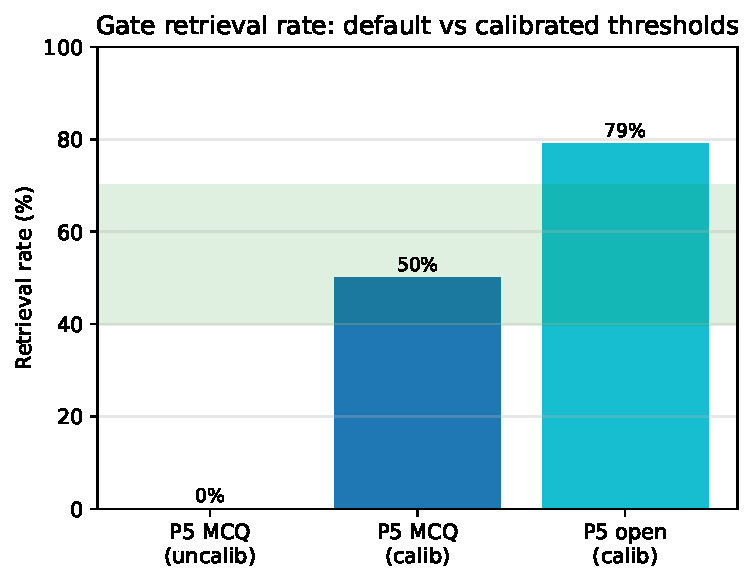
\includegraphics[width=0.75\linewidth]{results/figures/fig_retrieval}
  \caption{Gate retrieval rate before and after calibration. At default thresholds
  P5 retrieved on 0\% of queries; after calibration it retrieves at 50\% (MCQ) and
  79\% (open-ended), both within or above the 40--70\% target band (shaded).}
  \label{fig:retrieval}
\end{figure}

% ---------------------------------------------------------------------
\subsection{Open-Ended Evaluation}
\label{sec:open-ended}

All five MIRAGE subsets are multiple-choice, so the benchmark alone cannot test
free-text answering. The intended open-ended source (RAGCare-QA) was no longer
retrievable from its published location, so it was substituted with PubMedQA
(\texttt{pqa\_labeled}): 1{,}000 expert-annotated biomedical research questions,
each with a paragraph \emph{long answer}. This is genuine free-text question
answering, scored by token-level F1 (SQuAD-style) rather than letter matching, and
it exercises the hallucination probe's F1-agreement mode rather than its
letter-match mode. Both scoring and gating therefore branch correctly on question
type, verified end-to-end on the real data before any full run.

% ---------------------------------------------------------------------
\subsection{Results and the Headline Finding}
\label{sec:week3-results}

Table~\ref{tab:week3-results} reports all completed runs on the 200-question sets.
Two results stand out. First, calibration works exactly as designed: P5's
retrieval rate moves from 0\% to 50\% (MCQ) and 79\% (open-ended). Second, and
more consequentially, \emph{once P5 begins retrieving on the pilot corpus its
multiple-choice accuracy falls} from ccPthreeMcq{} (identical to closed-book, when it
never retrieved) to 45.5\%.

\begin{table}[t]
  \centering
  \begin{tabular}{lccccc}
    \toprule
    Policy & Type & $n$ & Acc.\ / F1 & Retrieval & Latency/q \\
    \midrule
    P1 always-retrieve   & MCQ  & 200 & 17.0\%          & 100\% & 12\,s \\
    P3 closed-book       & MCQ  & 200 & ccPthreeMcq   & 
etPthreeMcq & \latPthreeMcq \\
    P5 gated (uncalib.)  & MCQ  & 200 & ccPthreeMcq   & 0\%   & 142\,s \\
    P5 gated (calibrated)& MCQ  & 200 & 45.5\%          & 50\%  & 159\,s \\
    \midrule
    P3 closed-book       & open & 200 & 1PthreeOpen (F1) & 
etPthreeOpen & 27\,s \\
    P5 gated (calibrated)& open & 200 & 0.191 (F1)      & 79\%  & 171\,s \\
    \bottomrule
  \end{tabular}
  \caption{All completed 200-question runs (quantised Llama-3.2-3B, medium tier,
  200-chunk \emph{pilot} corpus). MCQ scored by accuracy, open-ended by mean
  token-F1. Latency is the mean wall-clock time per query.}
  \label{tab:week3-results}
\end{table}

This is not a bug but the central empirical finding: \textbf{gated retrieval
inherits the quality of the corpus it retrieves from}. The same effect explains
P1's very low 17.0\%: retrieving irrelevant context from a small pilot corpus
actively misleads the model relative to answering from its own parametric
knowledge, and the RAG prompt's instruction to rely on the provided context
compounds this. The gate is functioning correctly --- it fires at the calibrated
rate --- but on a weak corpus the act of retrieving is itself harmful. The
accuracy/latency frontier in Figure~\ref{fig:pareto} makes the trade-off concrete:
on the pilot corpus, closed-book (P3) dominates, being both cheaper and more
accurate than either retrieving policy.

\begin{figure}[t]
  \centering
  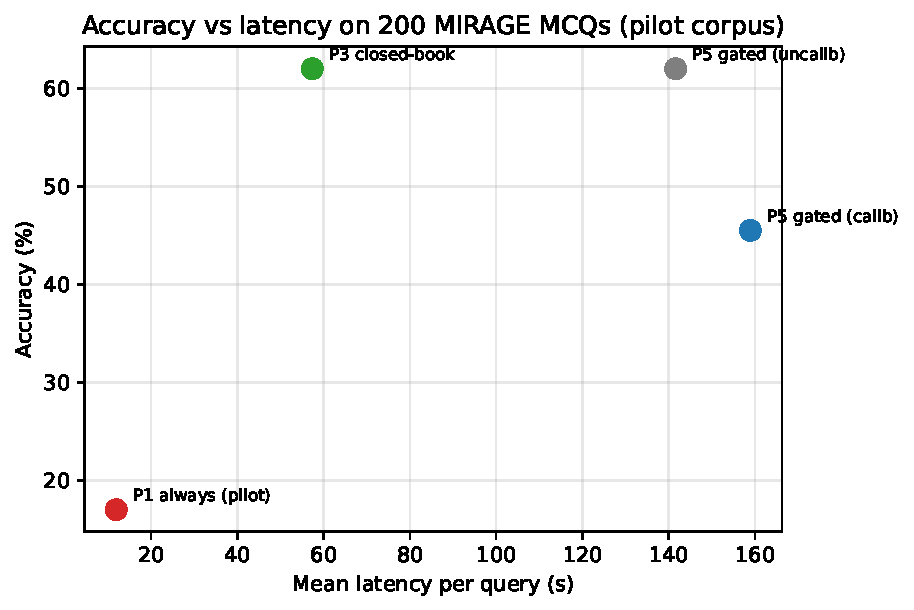
\includegraphics[width=0.8\linewidth]{results/figures/fig_pareto}
  \caption{Accuracy versus mean latency on 200 MIRAGE MCQs (pilot corpus). P3
  closed-book dominates the pilot-corpus frontier; the retrieving policies (P1,
  calibrated P5) pay a latency cost \emph{and} lose accuracy because pilot-corpus
  retrieval is unhelpful.}
  \label{fig:pareto}
\end{figure}

The practical consequence for the project is that the retrieval corpus, not the
gate, is now the critical variable: the gating machinery cannot be fairly evaluated
until it retrieves from a corpus that actually contains the answers. This directly
motivates the next phase --- replacing the pilot corpus with a real clinical
corpus (StatPearls / MedCorp) --- and reframes the safety-envelope analysis around
the corpus-quality dimension. It is also a genuinely useful negative result:
adaptive retrieval is only as safe as what it retrieves, and on a poor corpus the
safest gate is one that retrieves \emph{less}.

% ---------------------------------------------------------------------
\subsection{Summary}
\label{sec:week3-summary}

This sprint completed the retrieval engine (vector and hybrid retrievers),
implemented the remaining non-gated policies (P2, P4), and --- most importantly ---
calibrated the gate so that P5 performs genuine per-query routing. The full
cross-type comparison surfaced the project's headline finding: on the current
pilot corpus, retrieval degrades accuracy, so the corpus becomes the next
critical-path dependency. All figures and the results table are generated directly
from the logged per-query records, so the reported numbers and the plots share a
single source of truth.
